\documentclass{beamer}
\usepackage[frenchb]{babel}
\usepackage[OT1]{fontenc}
\usepackage[utf8]{inputenc}
\usepackage{indentfirst}
\usepackage{graphicx}
\usepackage{float}
\usepackage{colortbl}
\usepackage{color}
\usepackage{multimedia}
%\usetheme{Warsaw} 
\usecolortheme{orchid}
\usecolortheme{whale}
\hypersetup{pdfpagemode=FullScreen}
\usepackage{animate}
\usepackage{tdclock}
\usepackage{mathrsfs}
\usepackage{fancybox}
\usepackage{lmodern}
\usepackage{pdfpages} 
\usepackage{supertabular}
\usepackage{beamerthemeWarsaw}
%\usepackage{movie15}
\usetheme{AnnArbor}
%\usetheme{Antibes}
%\usetheme{Bergen}
%\usetheme{Berkeley}
%\usetheme{Berlin}
%\usetheme{Boadilla}
%\usetheme{CambridgeUS}
%\usetheme{Goettingen}
%\usetheme{Marburg}
%\usetheme{Montpellier} 
% %\usetheme{Singapore}
%\usetheme{Warsaw}
%\title[Astrophotographie]{Contribution au projet de recherche d'exoplanètes}
\author{\\EL HAMDAOUI Aicha }
%\institute{Master Physique des Hautes Énergies, Astrophysique et Physique Computationnelle}
\date{19 Juillet 2019}
\title{Transition de phase dans les trous noirs au delà de la relativité génerale}
\AtBeginSection[]{
	\begin{frame}
		\tableofcontents[currentsection]
	\end{frame}
}
\hypersetup{pdfborder={0 0 0},colorlinks,urlcolor=false,citecolor=black,linkcolor=black}
\renewcommand\thefootnote{\textcolor{black}{\arabic{footnote}}}
\newcommand{\reporttitle}{Transition de phase dans les trous noirs au delà de la relativité génerale}     % Titre
\newcommand{\reportauthor}{Aicha \textsc{EL HAMDAOUI}} % Auteur
\newcommand{\reportsubject}{\textbf{Mémoire}\\présenté pour obtenir le diplôme de master en: \\
\textbf{Physique des Hautes Énergies, Astrophysique et Physique computationnelle  }  } % Sujet
\newcommand{\HRule}{\rule{\linewidth}{0.7mm}}

\setbeamertemplate{navigation symbols}{}
\begin{document}

\begin{frame}
  \begin{minipage}{0.3\linewidth}
    	\begin{center}
    		%
\includegraphics[scale=0.44]{images/un.png}\\
    	\end{center}
   \end{minipage}\hfill
   \begin{minipage}{0.3\linewidth}
  	  	\begin{center}
  	  		%
\includegraphics[scale=0.14]{images/sem.png}\\
  	  	\end{center}
  \end{minipage}\hfill  
  \begin{minipage}{0.3\linewidth}
    	  	\begin{center}
    	  		%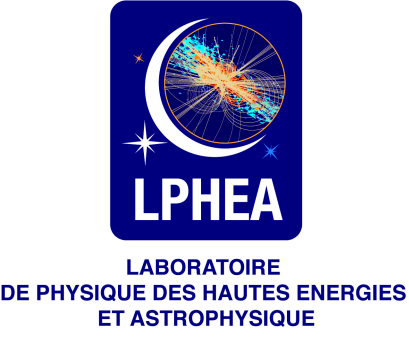
\includegraphics[scale=0.14]{images/labo.png}\\
    	  	\end{center}
    \end{minipage} 
 	\begin{center}
 	    { Université Cadi Ayyad} \\
 	     Faculté des Sciences Semlalia\\
 	    Laboratoire de Physique des Hautes Énergies et Astrophysique\\
 	    \textbf{Sous le thème}
 	    \end{center}
   
   \HRule
   \begin{center}
     \large  
     	\textcolor{blue}{\textbf{Transition de phase dans les trous noirs }} \\
     	\textcolor{blue}{\textbf{ au delà de la relativité génerale}}
   \end{center}
   \HRule
   \normalsize
   \newline
    \begin{minipage}[b]{0.45\linewidth}
          \begin{flushleft}
          \emph{Auteur :}\\
        \reportauthor
    \end{flushleft}       
       \end{minipage}
        \begin{minipage}[b]{0.45\linewidth}   
          \begin{flushright}
          		\begin{tabular}{l}
          			\textbf{Sous la direction de :} \\
          			       Mohamed \textsc{CHABAB} \\
          			        
          		\end{tabular}
              
    \end{flushright}   
       \end{minipage}
    
\end{frame}
%\begin{frame}
%\titlepage 
%\end{frame}

\begin{frame}
\tableofcontents[pausesections]
\end{frame}


\section{Les Trous Noirs En Astrophysique}
\subsection{Trous Noirs}

\begin{frame}
\begin{block}{Trou Noir }
	\begin{itemize}
	 	\item   un objet massif dont le champ gravitationnel est si
		intense qu’il empêche toute forme de matière ou de rayonnement de s'en échapper.
		\item    Objet astronomique céleste mystérieu .
	\end{itemize}
\end{block}
%\begin{column}{1cm}
%\includegraphics[scale=0.8]{image/trou.png}
%\end{column}

\end{frame}


\subsection{Formation des Trous Noirs}

\begin{frame}

%\begin{column}{1cm}
%\includegraphics[scale=0.55]{image/Capture2.png}
%\end{column}
\end{frame}

\subsection{Les differents types de Trous Noirs}

\begin{frame}

{Les differents type de Trous Noirs}


	\begin{itemize}
		\item Trous noirs stellaires.
		\item Trous noirs supermassifs.
		\item Trous noirs intermédiaires.
		\item Trous noirs primordiaux. 
	\end{itemize} 
\end{frame}


%
\subsection{Détection des Trous Noirs }
\begin{frame}{Détection des Trous Noirs}


\begin{block}{Trou noir dans un systéme binaire}
\begin{itemize}
	\item Repérage de l'accrétion du gaz de l'étoile compagnon:\\
	
	formantion d'un disque d'accrétion $\Rightarrow$ émission des rayons X $\Rightarrow$ détectable par les télescopes et satellites modernes .
	\item    Repérage grâce au mouvement de l'étoile compagnon:\\
	émission des ondes gravitationnelles $\Rightarrow$
	détecteurs interférométriques d'ondes gravitationnelles par LIGO  (1er détection 2015) .
\end{itemize}
\end{block}
	\begin{block}{Trou noir célibataire}
		\begin{itemize}
		\item l'effet de lentille gravitationnelle:\\
	déviation de la trajectoire des rayons lumineux  $\Rightarrow$ deux images identiques d'une m\^{e}me étoile située derrière le trou noir. 
		\item formantion d'un disque d'accrétion $\Rightarrow$ émission des rayons X $\Rightarrow$ reste  très théorique .

\end{itemize}
\end{block}
\end{frame}
\subsection{Propriétés des trous noirs}
\begin{frame}
\begin{block}{Propriétés des trous noirs}
un trou noir est entièrement connu par  trois caractéristiques: la masse, la charge électrique et le moment angulaire.
\end{block}


%	\begin{column}{6cm}
		%\includegraphics[scale=0.8]{image/Capture.png}	
%	\end{column}

\end{frame}

\section{ les Trous Noirs En Relativité générale}

\subsection{Les équations d'Einstein}

\begin{frame}
\begin{block}{Les équations d'Einstein}


\begin{itemize}
      \item une équation dynamique qui décrit comment la matière et l'énergie modifient la géométrie de l'espace-temps .
	\item l'équation la plus simple possible satisfaisant au principe d'équivalence . 
	\item  Elle redonne l'équation de Newton dans une limite appropriée (la limite non relativiste).
\end{itemize}
\end{block}
La forme mathématique de l'équation d'Einstein s'écrit :\\
$$R_{\mu\nu}-\dfrac{1}{2}Rg_{\mu\nu}+g_{\mu\nu}\Lambda=8\pi GT_{\mu\nu}$$

\end{frame}

\subsection{Le trou noir dans un espace asymptotiquement plat}
\begin{frame}
\begin{block}{la métrique de Schwarzschild}
	
	
	\begin{itemize}
		\item solution de l'équation d'Einstein dans le
		cas d'un champ gravitationnel isotrope.
		\item Sa métrique est donnéé par :
		$$ds^{2}=\left(1 -\dfrac{2GM}{rc^{2}} \right) c^{2}dt^{2}- \left(1 -\dfrac{2GM}{rc^{2}} \right)^{-1}dr^{2}-r^{2}d\theta^{2}-r^{2}sin^{2}(\theta) d\phi^{2}$$ 
		\item  La métrique montre deux singularitées pour deux valeurs de r différentes :
			\begin{itemize}
	\item	La coordonnée $ r=0$, o\`{u} la composante $g_{00}$ diverge.
		\item La coordonnée $ r = \dfrac{2GM}{c^{2}} = r_{s}$
		 (rayon de Schwarzschild), o\`{u} $g_{11}$ qui tend vers l’infinie.
	\end{itemize}
     \item La courbure scalaire donne l’expression suivante :
     $$R^{\mu\nu\alpha\beta}R_{\mu\nu\alpha\beta}=\dfrac{12r_{s}^{2}}{r^{6}}$$
	\end{itemize}

\end{block}
\end{frame}


%\subsection{Le trou noir dans un espace asymptotiquement plat}
\begin{frame}
\begin{block}{la métrique de Reissner Nordstrom}
	
	
	\begin{itemize}
		\item  solution de l'équation d'Einstein en présence de charge Q.
		$$R_{\mu\nu}-\dfrac{1}{2}g_{\mu\nu}R+g_{\mu\nu}\Lambda=8G\pi T_{\mu\nu}$$
		avec:
		$$T_{\mu\nu}=\dfrac{1}{4\pi}F_{\mu}^{\delta}F_{\nu\delta}-\dfrac{1}{4}g_{\mu\nu}F_{\alpha\beta}F^{\alpha\beta}$$
		\item Sa métrique est donnéé par :
		$$ds^{2}=-(1-\dfrac{2M}{r}+\dfrac{Q^{2}}{r^{2}})dt^{2}+(1-\dfrac{2M}{r}+\dfrac{Q^{2}}{r^{2}})^{-1}dr^{2}-r^{2}d\theta^{2}-r^{2}sin^{2}(\theta)d\phi^{2}$$ 
		\item  Sa métrique est singulière en:
		$$r_{\pm} = M \pm\sqrt{M^{2}-Q^{2}}$$
		
	\end{itemize}
	
\end{block}
\end{frame}

%\subsection{Le trou noir dans un espace asymptotiquement plat}
\begin{frame}
\begin{block}{la métrique de Kerr}
	
	
	\begin{itemize}
		\item  une solution exacte des équations d'Einstein permettant de décrire le comportement de l'espace-temps
		autour d'un trou noir en rotation $J\neq 0$ .
	
		\item Sa métrique est donnéé par :
			$$ds^{2}=-(1-\dfrac{2Mr}{\Sigma})dt^{2}+\dfrac{\Sigma}{\Delta}dr^{2}+\Sigma d\theta^{2}+\dfrac{Asin^{2}\theta}{\Sigma} d\phi^{2}-\dfrac{4Marsin^{2}\theta }{\Sigma} dt d\phi$$
			avec:
			
			$A=(r^{2}+a^{2})^{2}-\Delta a^{2}sin^{2}\theta$
		
			$\Sigma =r^{2}+a^{2}cos^{2}\theta$
			
			$\Delta=r^{2}-2Mr+a^{2}$
		\item  Sa métrique est singulière en:
		$$r_{\pm} = M \pm\sqrt{M^{2}-a^{2}}$$
		
	\end{itemize}
	
\end{block}
\end{frame}

%\subsection{Le trou noir dans un espace asymptotiquement plat}
\begin{frame}
\begin{block}{la métrique de Kerr-Newmann}
	
	
	\begin{itemize}
		\item  une solution de l'équation d'Einstein dans le cas d'un trou noir en rotation non chargé .
		
		\item Sa métrique est donnéé par :
		$$ds^{2}=-\dfrac{\Delta}{\rho^{2}}(dt-asin^{2}\theta d\phi)^{2}+\dfrac{sin^{2}}{\rho^{2}}[(r^{2}+a^{2})d\phi-adt]^{2}+\dfrac{\rho^{2}}{\Delta}dr^{2}+\rho^{2}d\theta^{2}$$
		où :
		
		$\Delta=r^{2}-2Mr+a^{2}+Q^{2}$\\
		et :\\
		$\rho^{2}=r^{2}+a^{2}cos^{2}\theta$ \\
		et finalement :\\
		$a=\dfrac{J}{M}$
	
		
	\end{itemize}
	
\end{block}
\end{frame}
\section{ LA THERMODYNAMIQUE DES TROUS	NOIRS}
\begin{frame}
 \textcolor{red}{violation du second principe de la thermodynamique} $\Leftrightarrow$ qui postule que cette grandeur est une fonction toujours croissante pour un système fermé or l'univers est un système fermé puisque rien ne peut en sortir par définition.$$\Downarrow$$ 
 cette disparition de l'entropie peut être évité si on considère l'entropie généralisée :
 $$S=S_{TN}+S_{ext}$$
 $$\Updownarrow$$ Bekenstein suggéra
 donc que l'entropie généralisé ne peut que croître.
 
\end{frame}
\subsection{Les quatre lois de la thremodynamique des trous noirs}
\begin{frame}
\begin{block}{Principe Zéro}
	
	La gravité de surface k d'un trou noir stationnaire est constante sur toute la surface de	l'horizon $ \Leftrightarrow$ La température T d'un corps est la m\^{e}me partout dans celui-ci  
	à l'équilibre thermique. 

\end{block}
\begin{block}{Premier Principe}
	$$dM=\dfrac{k}{8\pi}\delta A+\Omega_{h}\delta J+\Phi_{h}\delta Q$$ $$\Updownarrow$$  $$dE = T\delta S +\delta W$$
	 \\ 
	la variation de la masse entraîne une variation de l'énergie cinétique angulaire $\Omega_{h}\delta J$, une variation de l'énergie potentielle électrique $\Phi_{h}\delta Q$ et une variation d'énergie de rayonnement $\dfrac{k}{8\pi}\delta A$.
\end{block}

\end{frame}

%\subsection{Les quatre lois de la dynamique des trous noirs}
\begin{frame}
\begin{block}{Dexième Principe}
	
	 L'entropie d'un système isolé ne peut qu'augmenter $\delta S \geq 0$.$$\Updownarrow$$ L'air A de l'horizon des événements de chaque trou noir ne peut pas décroître $\delta A\geq 0$. 
	
\end{block}
\begin{block}{Troisième Principe}
	On ne peut atteindre $T = 0$ par aucun processus physique.$$\Updownarrow$$ On ne peut pas atteindre $k = 0$ par aucun processus.
\end{block}

\end{frame}

\subsection{Rayonnement du trou noir}
\begin{frame}
\begin{block}{Effet de Hawking}
un pair de particules crée prés de l'horizon d'un trou noir $\Rightarrow$ sous l'effet des forces de marées $\Rightarrow$ la particule d'énergie négative, tombe derrière l'horizon, et
la particule d'énergie positive restante peut s'éloigner à une grande distance du trou noir $\Rightarrow$ la particule ne pouvant plus se recombiner avec son antiparticule, elle va devenir réelle et appara\^{\i}tre à un observateur distant comme ayant été émise par le trou noir $\Rightarrow$ un appara\^{\i}tre d'un rayonnement d'évaporation en provenance du trou noir.
\end{block}
  	%\includegraphics[scale=0.8]{image/image.png}
\end{frame}

%\subsection{Rayonnement du trou noir}
\begin{frame}
\begin{block}{Température et Luminosité du trou noir}
	la température de Hawking en unités standard :
	$$T=\dfrac{\hbar c^{3}}{8\pi k_{b}GM}$$
	Avec $k_{b}$ est la constante de Boltzmann, $\hbar = \dfrac{h}{2\pi}$ (h
	est la constante de Plank ).\\
	
	la luminosité de rayonnement d'Hawking est donnée par:
	$$L=A\sigma T^{4}=\dfrac{\hbar c^{2}}{3840\pi r_{s}^{2}}=\dfrac{\hbar c^{6}}{15639\pi G^{2}M^{2}}$$
	Avec $\sigma = \dfrac{\pi^{2}k_{b}^{4}}{60\hbar^{3}c^{4}}$  est la constante de Stefan-boltzman.
\end{block}
\end{frame}
%\subsection{Rayonnement du trou noir}
\begin{frame}
\begin{block}{Durée de vie d'un trou noir}
	la durée de vie de trou noir de masse initiale M est égale :
	$$\tau=\dfrac{5120\pi G^{2}}{\hbar c^{4}}M^{3}$$
	Après les calculs des constantes, on obtien
    $$\tau = 10^{-16}M^{3}s.kg^{-3}$$
    est la durée de vie d'un trou noir une fois qu'il commence à s'évaporer.
\end{block}
\end{frame}
\section{THERMODYNAMIQUE DES TROUS NOIRS DANS UN ESPACE RN ADS}
	%\subsection{Thermodynamique du trou noir  AdS}
	\begin{frame}
Absence du terme $ P\delta V$ dans la
première loi $$\Downarrow$$ la pression peut \^{e}tre associée à une constante cosmologique négative$\Lambda$ .\\
pour les trous noirs asymptotiquement AdS
en quatre dimensions,on identifie la pression avec
$$P=-\dfrac{\Lambda}{8\pi}=\dfrac{3}{8\pi l^{2}}$$
Danc la première loi de la thermodynamique des trous
noirs rotatifs chargés dans un espace AdS s'écrit
$$dM=T\delta S+V\delta P+\Omega_{h}\delta J+\Phi_{h}\delta Q$$
\end{frame}

	\subsection{Thermodynamique du trou noir  AdS}

\begin{frame}
	A partire de $$g_{00}=1-\dfrac{2M}{r}+\dfrac{r^{2}}{l^{2}}$$
	On obtient :
	\begin{block}{La masse}
	$$	M=\dfrac{r_{h}}{2}(1+\dfrac{r_{h}^{2}}{l^{2}})$$
		
	\end{block}
	\begin{block}{ Premier principe de la thermodynamique }
$	dM=TdS+VdP $
	
\end{block}
\begin{block}{ Temperature }
$$T=(\dfrac{\partial M}{\partial S})_{P}=\dfrac{1}{4\pi}(1+\dfrac{3r_{h}^{2}}{l^{2}})$$
	
\end{block}
	\begin{block}{vérification de la relation de Smarr}
		$$M=2TS-2PV$$
	
\end{block}
\end{frame}
%\subsection{Thermodynamique du trou noir  AdS}
\begin{frame}
\begin{block}{l'énergie libre de Gibbs G }
G $\Rightarrow$	informations sur la stabilité thermodynamique
$$G=M-TS=\dfrac{r_{h}}{4}(1-\dfrac{r_{h}^{2}}{l^{2}}),$$
avec $$M\equiv H$$
\end{block}
\textcolor{red}{L'énergie libre de Gibbs en fonction de T , l = 1}
	%\includegraphics[scale=0.5]{image/GT.png}
\end{frame}
%\subsection{Thermodynamique du trou noir  AdS}
\begin{frame}
On peut résumée ces phases selon les conditions suivantes :
	
\begin{itemize}
	\item  Pour $ T < T_{m}$, seulement la phase rayonnement thermique pure qui existe.
	
	\item Pour $T_{m} < T < T_{HP}$ , on a $G_{rayonement} < G_{trounoir}$, la phase rayonnement thermique est
	plus stable et donc plus dominante.
	
	\item Pour $T > T_{HP}$ , on a $G_{rayonement} > G_{trounoir}$, la phase large trou noir c'est la plus stable et la pus dominante.\\
	avec:
	$$\dfrac{\partial T}{\partial r_{h}}=0 \Leftrightarrow T_{m}=\dfrac{\sqrt{3}}{2\pi l},$$
	et
	$$G=0 \Leftrightarrow T_{HP}=\dfrac{1}{\pi l}.$$
	
	
\end{itemize}

\end{frame}

%\begin{frame}
%\textcolor{red}{La ligne de coexistence des deux phases : rayonnement thermique/large trou noir}
%\large  $$P_{HP}=\dfrac{3\pi}{8}T_{HP}^{2}$$
%\end{frame}



\begin{frame}
\begin{block}{Chaleur spécifique à pression constante C{p}}
	$$C_{p}=\left( \dfrac{\partial M}{\partial T}\right) _{p}=-\dfrac{2\pi r_{h}^{2}(1+8\pi Pr_{h}^{2})}{-1+8\pi Pr_{h}^{2}}$$
\end{block}

\begin{columns}
	\begin{column}{5cm}
		%\includegraphics[scale=0.45]{image/Cp.png}
	\end{column}
	\begin{column}{7cm}
		
		\begin{block}{La stabilité et la chaleur spécifique}
			\begin{itemize}
				\item $C_{p}$ a une asymptote verticale au point $r_{h} = \dfrac{l}{\sqrt{3}} =r_{hm} \Leftrightarrow T=T_{m}$
				\item $r_{h} < r_{hm} \Leftrightarrow  T < T_{m} $ la chaleur spécifique est négative, dans ce cas le système thermodynamique est instable .
				\item $r_{h} > r_{hm} \Leftrightarrow  T > T_{m} $ la chaleur spécifique est positive, donc c’est la région stable.
				
			\end{itemize}
		\end{block}
	\end{column}
\end{columns}
\end{frame}
\subsection{Thermodynamique du trou noir RN AdS}
\begin{frame}
A partir de 
$$g_{00}=1-\dfrac{2M}{r}+\dfrac{Q^{2}}{r^{2}}+\dfrac{r^{2}}{l^{2}}$$
On obtient :
\begin{block}{La masse}
$$M=\dfrac{1}{2} \left( r_{h}+\dfrac{Q^{2}}{r_{h}}+\dfrac{8\pi}{3}r_{h}^{3}P\right)$$
\end{block}
\begin{block}{Temperature}
$$T=(\dfrac{\partial M}{\partial S})_{Q,P}=T=\dfrac{1}{4r_{h}\pi}(1-\dfrac{Q^{2}}{r_{h}^{2}}+8\pi Pr_{h}^{2})$$
\end{block}
\begin{block}{Pression}
$$P=\dfrac{T}{2r_{h}}-\dfrac{1}{8\pi r_{h}^{2}}+\dfrac{Q^{2}}{4\pi r_{h}^{4}}$$
\end{block}

\end{frame}
%\subsection{Thermodynamique du trou noir RN AdS}
\begin{frame}
\begin{block}{l'equation de l'état}
$$\nu=2l_{p}^{2}r_{h}$$ $$\Downarrow$$ $$P=\dfrac{T}{\nu}-\dfrac{1}{2\pi \nu^{2}}+\dfrac{2Q^{2}}{\pi \nu^{4}}$$
\end{block} 
cette équation présente un comportement
critique et une point d'inflexion qui se produit lorsque 
$$\dfrac{\partial P}{\partial \nu}=0 $$ et $$\dfrac{\partial^{2} P}{\partial \nu^{2}}=0$$ 
\end{frame}
%\subsection{Thermodynamique du trou noir RN AdS}
\begin{frame}
On obtient alors les coordonnées du point critique
\begin{block}{Points Critiques}
$$P_{c}=\dfrac{1}{96\pi Q^{2}}$$
$$\nu_{c}=2\sqrt{6}Q$$
$$T_{c}=\dfrac{\sqrt{6}}{18\pi Q}$$
\end{block}


$$\Downarrow$$
$$\dfrac{P_{c}\nu_{c}}{T_{c}}=\dfrac{3}{8}$$
 \textcolor{red}{C'est un nombre universel
 	pour tout les trou noir de RN-AdS}.

\end{frame}
%\subsection{Energie libre de Gibbs et la température de coexistence}
\begin{frame}
$$G=\dfrac{1}{4}\left(\dfrac{\nu}{2}-\dfrac{\pi}{3}P\nu^{3}+\dfrac{6Q^{2}}{\nu} \right)$$

		%\includegraphics[scale=0.9]{image/gtrn.png}
	\end{frame}
\begin{frame}
		
		\begin{block}{$G-T$}
			\begin{itemize}
				\item $P<P_{c} $ l'allure de G montre une transition de phase du premier ordre. $\Rightarrow$ l'équation d’état produit trois racines réelles .
				
				\item $P = P_{c}$ la transition de phase est de deuxième ordre, l'équation d’état produit une
				seule racine réelle "double" .
				\item $P > P_{c}$ l'équation d'état ne produit qu'une seule racine réelle, le système n'est
				stable que sous une seule phase, c'est une phase supercritique.
				
			\end{itemize}
		\end{block}
	
\end{frame}
%\subsection{La stabilité et la chaleur spécifique}
\begin{frame}
\textcolor{red}{la chaleur spécifique :} 
$$C_{p}=\dfrac{2\pi^{2}\nu^{6}P-4\pi \nu^{2}Q^{2}+\pi \nu^{2}}{4\pi \nu^{4}P-2\nu^{2}+24Q^{2}}$$
\pause
	%\includegraphics[scale=0.5]{image/cprn.png}
		\pause
\begin{itemize}
	\item $P<P_{c} $ $\Rightarrow$ $C_{p}$ est
	toujours positive pour les petits trous noirs $ \nu <\nu_{max} $ et larges trous noirs $ \nu > \nu_{min}$ .
		\end{itemize}
	

	
	\end{frame}
	\begin{frame}
	
		%\includegraphics[scale=0.5]{image/psuppc.png}
	\begin{itemize}
		\item $P>P_{c} $ $\Rightarrow$ $C_{p}$  ne diverge pas et elle est toujours positive $\Rightarrow$ une seule phase qui est la phase "large trou noir" .
	\end{itemize}

	


\end{frame}

\begin{frame}
	%\includegraphics[scale=0.5]{image/pegalpc.png}
\begin{itemize}
\item $P=P_{c} $ $\Rightarrow$ $C_{p}$  admet une seule asymptote verticale en $\nu_{c}$.
\end{itemize}
\end{frame}
\subsection{Géométrie thermodynamique et transition de phase}
%\subsection{Métrique de Ruppeiner}
\begin{frame}
\textcolor{red}{Géométrie thermodynamique}:\\
Est une autre approche pour étudier le comportement thermodynamique
du systéme .  
\begin{itemize}
\item Métrique de Ruppeiner.
\item Métrique de Quevedo .
\item Métrique de HPEM .
\end{itemize}

\end{frame}
\begin{frame}
\textcolor{red}{Métrique de Ruppeiner}
	%\includegraphics[scale=0.5]{imag/metriqueR.png}

\begin{block}{}
Nous pouvons remarquer que le point de divergence n’est pas identique à celui de la
capacité thermique $(S_{min}, S_{max})$ pour $P < P_{c}$ et Sc pour $ P = P_{c}$. Par conséquent,
c'est à dire 
que le point de divergence n'est pas identique à la divergence / point zéro de la capacité calorifique, c'est pourquoi
Métrique n'est pas en mesure de décrire la transition de phase de cette solution de trou noir.
\end{block}
\end{frame}
%\subsection{Métrique de Quevedo}

\begin{frame}
\textcolor{red}{Métrique de Quevedo}
%\includegraphics[scale=0.5]{imag/metriqueQ.png}

\begin{block}{}
	Il est clair que cette métrique présente des points de divergence qui coïncident avec
	ceux de la capacité thermique. On peut dire que cette géométrie est capable de décrire la
	transition de phase 1er/2ème ordre pour les trous noirs de RN-AdS.
\end{block}
\end{frame}
%\subsection{Métrique de HPEM}

\begin{frame}
\textcolor{red}{Métrique de HPEM}
%\includegraphics[scale=0.5]{imag/matriqueH.png}
\begin{block}{}
	On peut voir que les points de divergence coïncident exactement avec les points de
	divergence de la capacité calorifique ainsi que son point zéro. Alors on peut dire que cette
	métrique peut décrire la transition de phase et déterminer le trou noir extrémal donné
	par $C_{p} = 0$ ou T = 0.\\
\end{block}
\end{frame}
\section{Conclusion}
\begin{frame}
\begin{block}{Conclusion}
\begin{itemize}
	\item La physique de Newton ne donne pas toujours des résultats
	satisfaisants. Pour étudier les trous noirs, il faut penser au
	relativité générale.
	\item Un trou noir est un astre dont la vitesse de libération est plud grand que la vitesse de la lumière de sorte que rien ne se que échappé.
	\item le scénario de Hawking-Page , les trous noirs de Schwarzschild dans
	l’espace anti-de Sitter présente une transition de phase thermodynamique .
	\item Le trou noir RN-AdS présente un comportement
	thermodynamique similaire à celui d’un fluide de
	Van-der-Wals .
	\item La capacité thermique $ C_{p}$
	permette d'étudier la stabilité et les points critiques .
	\item  la géométrie thermodynamique est Une autre approche pour étudier le comportement thermodynamique des trous noirs.
\end{itemize}
\end{block}

\end{frame}

\end{document}

